Menu rozruchowe (boot menu) służy do wskazywania który z zainstalowanych systemów operacyjnych ma zostać uruchomiony podczas rozruchu komputera. Jeżeli zainstalowałeś Ubuntu jako jedyny system operacyjny, to menu rozruchowego nie zobaczysz. Można je wyświetlić poprzez wciśnięcie klawisza \keys{Shift} lub \keys{\arrowkeydown} w chwili pojawienia się fioletowych pasów na krawędziach ekranu. Jeżeli masz więcej niż jeden system operacyjny, ekran rozruchowy programu GRUB zostanie wyświetlony i rozpocznie się odliczanie, po upływie którego zostanie wybrana pierwsza pozycja z listy.

Konfiguracja wyglądu i zachowania menu rozruchowego jest możliwa, ale wymaga bardzo dobrej znajomości dokumentacji programu GRUB i umiejętnego stosowania wiersza poleceń. To wykracza daleko poza zakres tego Przewodnika. Zamiast tego, posłużymy się programem \textcolor{ubuntu_orange}{Grub Customizer}. Aby go zainstalowac wykonaj:
\begin{lstlisting}[language=bash]
sudo add-apt-repository ppa:danielrichter2007/grub-customizer
sudo apt-get update
sudo apt-get install grub-customizer
\end{lstlisting}

\begin{wrapfigure}[7]{R}{0.5\textwidth}
	\vspace{-10pt}
	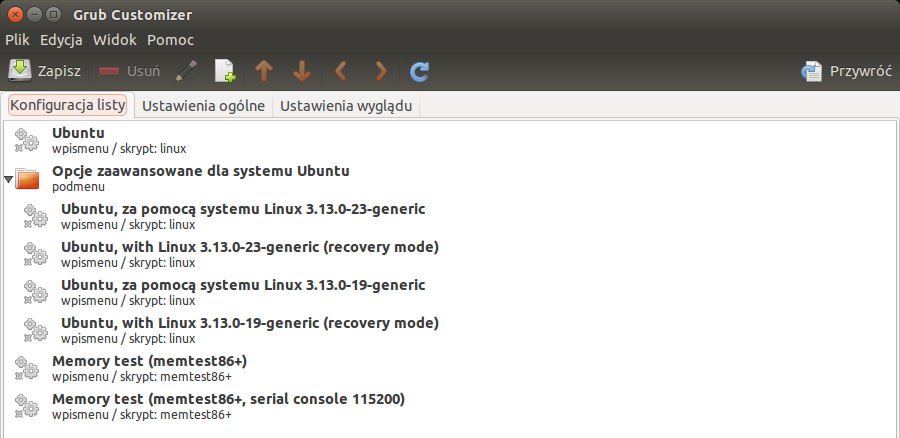
\includegraphics[width=\linewidth]{images/programy_grub_customizer.png}
\end{wrapfigure}

Teraz uruchom program Grub Customizer. Zmiany w menu rozruchowym wymagają uprawnień administratora, więc zostaniesz poproszony o podanie hasła. Kiedy to zrobisz, program przeskanuje aktualną konfigurację i wyświetli swoje okno. Dostępne są w nim trzy zakładki:
\vspace{0.1cm}
\begin{itemize}
\item \textcolor{ubuntu_orange}{Ustawienia listy} --- służy do konfiguracji kolejności elementów na liście. Pierwszy element zostanie domyślnie wybrany podczas rozruchu systemu. Elementy usunięte z tej listy nie pojawią się w menu GRUB-a, widocznym podczas uruchamiania komputera (co może skutkować niemożliwością uruchomienia systemu w ogóle).
\item \textcolor{ubuntu_orange}{Ustawienia ogólne} --- służy do zmiany podstawowych parametrów.
\item \textcolor{ubuntu_orange}{Ustawienia wyglądu} --- pozwala zmienić kolory i rozmiar menu rozruchowego, a także wgrać tapetę.
\end{itemize}

W programie dostępny jest jeszcze przycisk \textcolor{ubuntu_orange}{Zaawansowane}. Włącza on menu ustawień przeznaczonych dla doświadczonych administratorów systemu.

Aby zapisać wprowadzone przez siebie zmiany, kliknij przycisk \textcolor{ubuntu_orange}{Zapisz}, znajdujący się na górnej belce narzędziowej.
\clearpage
